\section{CCP and background}\label{sec:ccp}

\subsection{Background}

We worked on this project in conjunction with CCP Games. The project was a continuation of work done by Reykjavík University graduates Gunnar Þór Stefánsson and Þór Adam Rúnarsson. They worked on it as their final project for the spring semester of 2015. They continued their work with a grant from Rannís during the summer of 2015. Gunnar had to leave the project in the beginning of July and Hjalti Leifsson replaced him. 

When the project began, a user interface design had been decided, and the game had around half of that design already implemented. The design can be seen on figure \ref{fig:PD}.

\begin{figure}[H]
	\centering
	\graphicspath{ {./graphics/} }
    \centerline{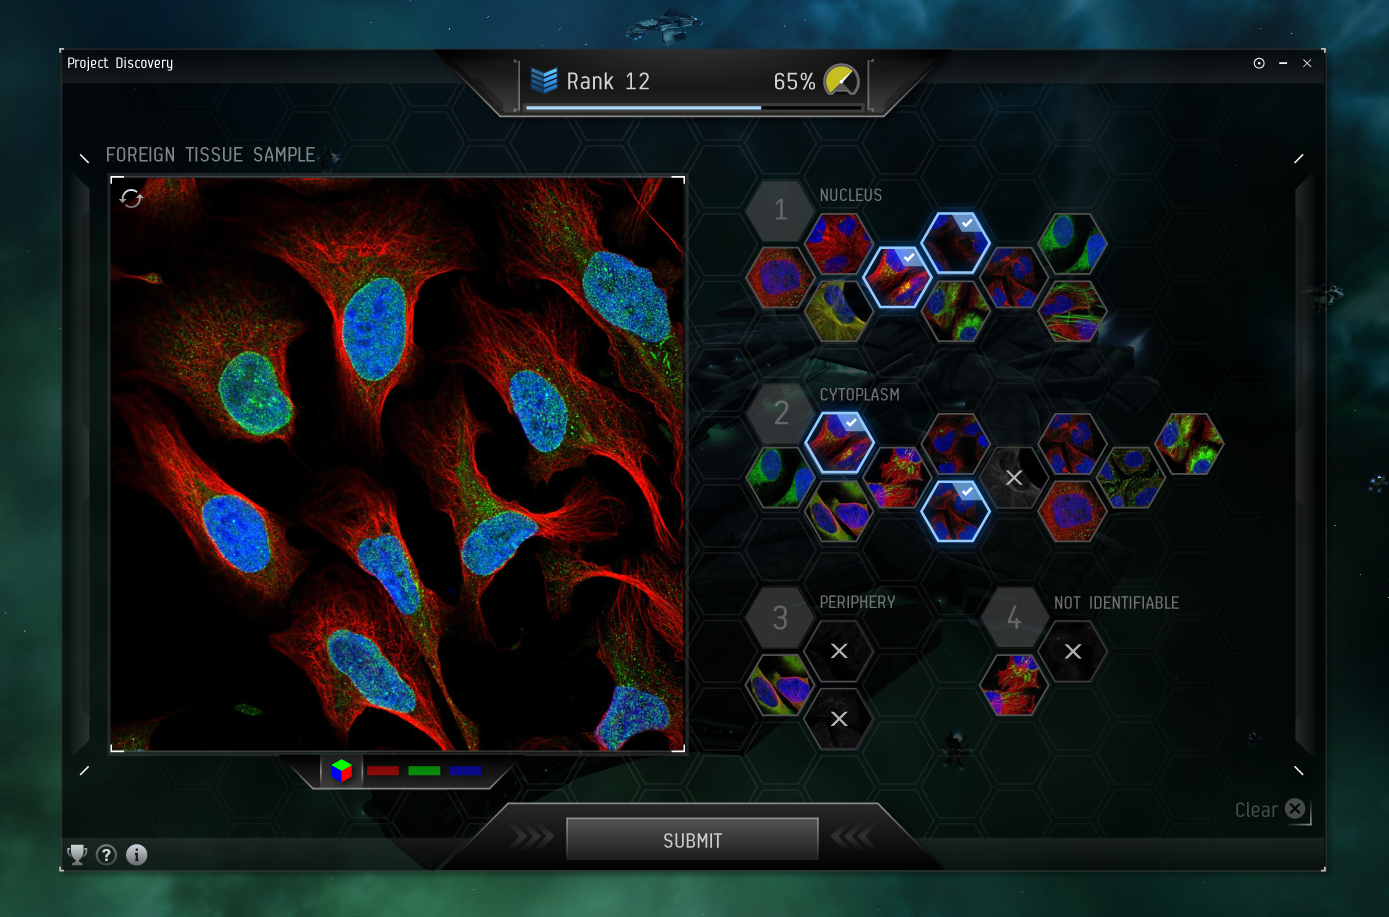
\includegraphics[scale=0.35]{PD.png}}
    \caption{\label{fig:PD}The design of the UI as the project began}
\end{figure}

The game already had a few features implemented, such as players being able to receive images, selecting their appropriate categories and submitting their classifications. A simple rewarding system was also already in place, rewarding players with in game currency (ISK), experience points (XP) and loyalty points (LP) when players submitted a solution. The reward was based on their score for the image they just classified, but since those images were 'training images', we knew the solution and could grade the player on that. However, that needed to be changed later on because when the client got an image that we did not know the solution for, no reward was given. Finally, a rudimentary tutorial phase was implemented, but it was too small and needed to be expanded to improve new player experience.

\subsection{CCP Games}

CCP develops massively multiplayer online games and has become one of the leading companies in that field. It is dedicated to make original, cutting edge games. CCP is best known for their groundbreaking massively multiplayer online role-playing game (MMORPG) \emph{EVE Online}, which has enjoyed great popularity and received critical acclaim, winning Game of the Year three times from \href{http://www.mmorpg.com/}{MMORPG.com}. In addition to \emph{EVE Online}, CCP also develops \emph{DUST 514\textsuperscript{\textregistered}}, an innovative, free-to-play, massively multiplayer online first-person shooter for the PlayStation\textsuperscript{\textregistered}3, and \emph{EVE: Valkyrie™}, a multiplayer spaceship dogfighting shooter, both set in the EVE Universe. CCP was founded in Reykjavík Iceland in 1997. Its headquarters have since recided there but it also has locations in Atlanta, Newcastle and Shanghai. Further information can be found at \href{http://www.ccpgames.com/}{CCPGames.com}.

CCP provided us with facilities to work on the project, and their game \emph{EVE Online} accomodates Project Discovery within its game universe. We had a project manager, Pétur Örn Þórarinsson, from CCP to help us work with the company. 

\subsection{EVE Online}
\emph{EVE Online} is the game which plays host to \emph{Project Discovery}. It is based in a science fiction space setting. Players of the game have a great deal of freedom in how they choose to play and don't need to follow pre-defined missions. They can engage in many different activities such as mining, piracy, manufacturing, trading, exploration and combat (both player versus environment and player versus player). \emph{Project Discovery} fits smoothly into the game as players can solve tasks from anywhere in the game. To access \emph{Project Discovery}, players go through the menu and select it, and a new window opens up on the game screen.
